\documentclass{article}

\usepackage{tikz}
\usepackage{tikz}
\usepackage{pgfplots}
\usetikzlibrary{backgrounds, positioning, fit}
\usetikzlibrary{shapes.geometric}
\usetikzlibrary{patterns}

%% put tikzlibrary below if necessary

% set up externalization
\usetikzlibrary{external}
\tikzset{external/system call={latex \tikzexternalcheckshellescape -halt-on-error
-interaction=batchmode -jobname "\image" "\texsource";
dvips -o "\image".ps "\image".dvi;
ps2eps "\image.ps"}}
\tikzexternalize


\begin{document}


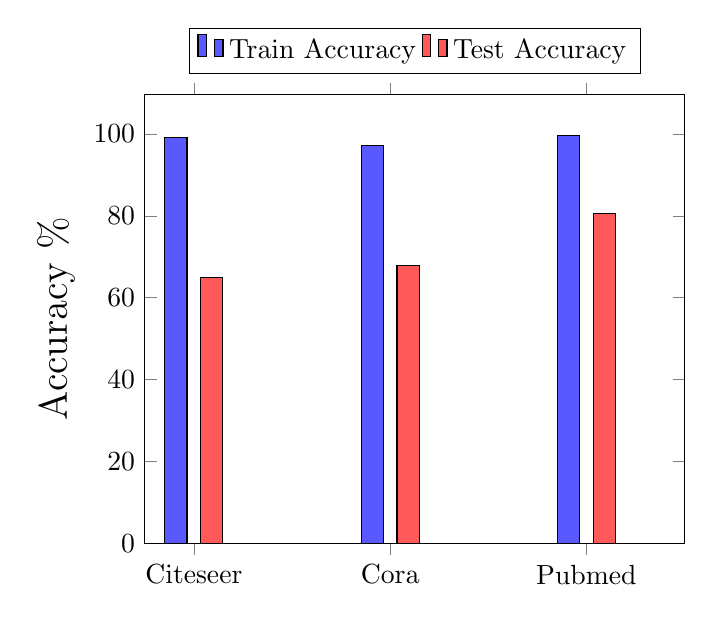
\begin{tikzpicture}
\begin{axis}[
ylabel=Accuracy \%,
%ylabel style={yshift=-1cm},
%xlabel=,
xtick={0,1,2,3},
xticklabels={,Citeseer,Cora,Pubmed},
%xlabel style={yshift=0.35cm},
legend style={at={(0.5,1.15)},anchor=north,legend columns=-1,font=\normalsize},
ybar=5pt,% configures ‘bar shift’
bar width=8pt,
ylabel near ticks,
xlabel near ticks,
x label style={font=\Large},
y label style={anchor=south,font=\Large},
ytick style={font=\large},
xtick style={font=\large},
xmax=3.5,
ymin=0
]

\addplot [fill=blue!65] coordinates {(1,99.24) (2,97.22) (3,99.61)};
\addplot [fill=red!65] coordinates {(1,64.95) (2,67.89) (3,80.59)};


\legend{Train Accuracy, Test Accuracy}
\end{axis}


\end{tikzpicture}



\end{document}
